% ísticos que baseiam-se na %--------------------------------------------------------------------------------------
% Este arquivo contém a sua metodologia
%--------------------------------------------------------------------------------------
\chapter{Materiais e Métodos} \label{ch:MateriaisMétodos} %Uma label é como você referencia uma seção no texto com a tag \ref{}
    % Neste capítulo será apresentado como será feita a avaliação do desempenho das funções de ranqueamento na Mineração de Texto.
    Este capítulo apresenta o modo de avaliação do desempenho dos atributos, gerados a partir da função de ranqueamento BM25, em Mineração de Texto.
    A metodologia proposta está ilustrada na Figura \ref{fig:diagrama-da-metodologia} e o processo é detalhado a seguir.
    
    \begin{figure}[H]
    \centering
    \caption{Metodologia proposta para avaliação de desempenho, em verde estão as variáveis mensuráveis sugeridas.}
    \begin{center}
        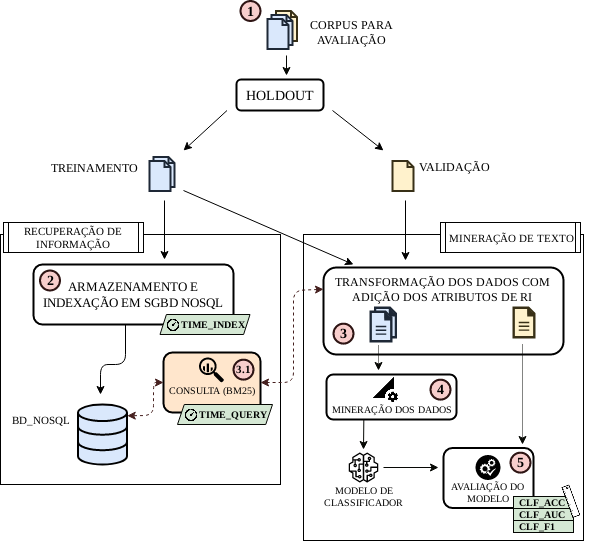
\includegraphics[width=0.8\textwidth]{img/diagrama-metodologia-v2-2.png}
    \end{center}
    \vspace{-0.5cm}
    \legend{\ABNTEXfontereduzida \textbf{Fonte:} O autor.}
    \label{fig:diagrama-da-metodologia}
\end{figure}
    
    Inicialmente é necessário selecionar os \textbf{(1) Corpus para Avaliação} que servem para efetuar as avaliações de desempenho, e, caso esses corpus ainda não estejam segmentados em exemplos para treinamento e exemplos para validação, é feita essa separação com o método de \textit{holdout}\footnote{Particionamento aleatório do dados em dois conjuntos independentes, geralmente chamados de treinamento e teste. O conjunto de treinamento é utilizado para derivar o modelo e o de teste para estimar a sua acurácia. \cite[p.~370]{Han:2011:DMC:1972541}.} de $\frac{2}{3}$ para treinamento e $\frac{1}{3}$ para validação.
    
    Em seguida, o conjunto de treinamento passa pela fase de RI, aonde é feito o \textbf{(2) Armazenamento e Indexação em  SGBD NoSQL} por meio das ferramentas apresentadas na Seção  \ref{sec:Armazenamento-e-indexação}, sendo mensurado o tempo necessário para concluir essa operação em cada um dos Sistemas Gerenciadores de Banco de Dados (SGBD) NoSQL selecionados.
    
    O processo de Mineração de Texto pode ser segmentado em 7 etapas, conforme ressaltado anteriormente na Seção \ref{sec:MineraçãoTexto}.
    Na metodologia proposta aqui a fase de MT assume que as 3 etapas iniciais de limpeza, integração, e seleção dos dados, já foram realizadas no banco de dados de teste, assim os conjuntos divididos em treinamento e validação passam diretamente pela etapa seguinte que é a \textbf{(3) Transformação dos dados com adição dos atributos de RI}.
    Nesta etapa, os banco de dados NoSQL indexados recebem \textbf{(3.1) Consultas} com a utilização das funções de ranqueamento baseadas no BM25 que cada ferramenta implementa, sendo mensurado o tempo para efetuar cada consulta e gerar os novos atributos sugeridos adiante na Seção \ref{sec:Atributos-de-RI-sugeridos}.
    % Será feita uma consulta para cada exemplo dos conjuntos, e a resposta dessas consultas servirá para criar os atributos de RI detalhados logo mais na Seção \ref{sec:Atributos-de-RI-sugeridos}.
    
    O processo de \textbf{(4) Mineração dos Dados} é feito por meio da réplica de soluções dos corpus para avaliação selecionados, que possuem seus códigos-fonte disponíveis, sendo então reproduzida cada solução 
    \begin{enumerate*}[label=(\alph*)]
        \item sem nenhuma alteração, e 
        \item com adição dos novos atributos sugeridos.
    \end{enumerate*}
    Esse processo gera dois modelos de classificador, o primeiro criado sem atributos de RI e o segundo com esses atributos.
    A etapa de \textbf{(5) Avaliação do Modelo} permite que para cada modelo sejam geradas medidas da literatura de MT, detalhadas logo mais na Subseção \ref{subsec:Desempenho-de-classificador}, a partir do teste com o conjunto de validação, possibilitando a comparação do ganho de desempenho de classificador com/sem atributos de RI.
    % Na fase de Mineração de Texto os conjuntos de treinamento e de validação passarão pela \textbf{(3) Transformação dos dados com adição dos atributos de RI} onde 
    
    
    % Para utilização da função de ranqueamento BM25 como variável em tarefas de mineração de texto é necessário efetuar o armazenamento e a indexação dos textos do conjunto de treinamento, e para esta tarefa serão utilizadas ferramentas de armazenamento em banco de dados (não relacionais?) que fornecem implementações do BM25 para consulta, estas serão apresentadas na Seção \ref{sec:Armazenamento-e-indexação}.
    
    % Se faz necessário também definir medidas para avaliação do ganho de desempenho com as variáveis de RI, assim como elencar as bases de dados que vão servir para efetuar essa avaliação, disposto logo mais nas Seções \ref{sec:Medidas-para-avaliação-de-desempenho} e \ref{sec:Corpus-para-avaliação}.

\section{Corpus para avaliação}  \label{sec:Corpus-para-avaliação}
    Foram definidos dois corpus de competições promovidas pela PAN, sigla da organização que se originou do \textit{International Workshop on Plagiarism Analysis, Authorship Identification, and Near-Duplicate Detection} em 2007 \cite{PAN_Workshop_2007}, sendo estes descritos a seguir:% https://web.archive.org/web/20190711212207/https://www.uni-weimar.de/medien/webis/events/pan-07/pan07-web/
    
    % Os banco de dados de teste selecionados para avaliação são os utilizados na PanCLEF 2019 % necessário citar a PanCLEF anteriormente
    \begin{itemize}
    % Author Profiling - PAN @ CLEF 2018
    % Soluções disponíveis:
    % 2. daneshvar18 - https://github.com/SamanDaneshvar/pan18ap
    %  https://pan.webis.de/downloads/publications/papers/daneshvar_2018.pdf
    % 4. laporte18 - https://github.com/arthur-sultan-info/PAN2018-AP
    % https://pan.webis.de/downloads/publications/papers/ciccone_2018.pdf
    % 12. gouravdas18 - https://github.com/brajagopalcse/PAN2018
    % https://pan.webis.de/downloads/publications/papers/gopalpatra_2018.pdf
    % 16. schaetti18 - https://github.com/nschaetti/PAN18-Author-Profiling
    %  https://pan.webis.de/downloads/publications/papers/schaetti_2018a.pdf
    % 21. raiyani18 - https://github.com/kraiyani/author-profiling-pan-clef-2018 
    % https://pan.webis.de/downloads/publications/papers/raiyani_2018.pdf
    % 23. jucikarlgreen - https://github.com/jussikarlgren/pan18
    % https://pan.webis.de/downloads/publications/papers/karlgren_2018.pdf
        \item \textbf{DB\underscore{}AUTHORPROF - \textit{Author Profiling - PAN @ CLEF 2018}:} Uma tarefa da competição \textit{CLEF 2018} promovida pela PAN na classe de análise de autoria, a qual foca na identificação de gênero no Twitter em três linguagens distintas, inglês, espanhol, e árabe \cite{PAN_APCLEF_2018}.
        
        Os dados consistem de 100 \textit{tweets}\footnote{Termo utilizado para designar as publicações feitas na rede social do Twitter.} e 10 imagens para cada autor, sendo que o conjunto de treinamento possui \begin{enumerate*}[label=(\alph*)]
            \item 3000 autores em inglês, \item 3000 autores em espanhol, e \item 1500 autores em árabe,
        \end{enumerate*}
        e o conjunto de validação possui
        \begin{enumerate*}[label=(\alph*)]
            \item 1900 autores em inglês, 
            \item 2200 autores em espanhol, e 
            \item 1000 autores em árabe
        \end{enumerate*}
        \cite{rangel2018overview}.
        
        Segundo \citeonline{rangel2018overview} esse banco de dados da \textit{CLEF 2018} com um total de 12600 autores é um subconjunto da tarefa de \textit{Author Profiling} da \textit{CLEF 2017} e eles foram classificados em dois passos,
        \begin{enumerate*}[label=(\roman*)]
            \item automaticamente com a ajuda de um dicionário de nomes próprios, e
            \item manualmente verificando a foto, descrição e outros elementos de cada perfil
        \end{enumerate*}
        \cite{rangel2017overview}.
        
        % \item \textbf{DB\underscore{}BOTGENDER - \textit{Bots and Gender Profiling PAN @ CLEF 2019}:}
        % https://pan.webis.de/clef19/pan19-web/author-profiling.html
        % 7 - Ipsas & Popescu - https://github.com/adiIspas/Bots-Gender-Profiling
        % 10 - Goubin - https://github.com/pan-webis-de/goubin19
        % 11 - Polignana & de Pinto - https://github.com/pan-webis-de/polignano19
        % 23. De La Peña & Prieto - https://github.com/JoseRPrietoF/autoria
        % 30. Rahgoyu - https://github.com/HamedBabaei/PAN2019_bots_gender_profiling
        % 32 Pryzybyla Przybyła - https://github.com/pan-webis-de/przybyla19
        
        \item \textbf{DB\underscore{}HYPARTISAN - \textit{Hyperpartisan News Detection - PAN @ SemEval 2019 Task 4}:} Esta tarefa da competição \textit{SemEval 2019} promovida pela PAN consiste em, dada uma notícia, avaliar se esta segue uma argumentação hiperpartidária, que significa verificar se ela possui fidelidade cega, preconceituosa, ou irracional a um partido, grupo, causa, ou pessoa \cite{PAN_HND_2019}.
        Portanto pode-se dizer que se trata de um problema de classificação binária, a classe real é a presença ou ausência de hiperpartidarismo em cada exemplo.
        
        Os dados consistem em artigos de notícias divididos em múltiplos arquivos onde cada arquivo com parte inicial ``articles-'' consiste em uma notícia e a classificação real da notícia está presente em um arquivo com inicial ``ground-truth-''. 
        Além disso os dados estão divididos em duas partes, a primeira composta de 750 mil artigos está classificada pelo enviesamento geral do editor, onde metade está classificada como hiperpartidária e a outra metade não. 
        Dessa parte, 80\% (600 mil artigos) estão no conjunto de treinamento e 20\% (150 mil) estão no conjunto de validação, sendo que nenhum editor de artigos do conjunto de treinamento se repete no conjunto de validação \cite{johannes_kiesel_2018_1489920}.
        
        A segunda parte dos dados foi rotulada através de \textit{crowdsourcing}\footnote{Obter entrada para uma tarefa ou projeto específico contando com os serviços de um número de pessoas, pagas ou não, tipicamente através da Internet.}. 
        Essa parte dos dados contêm um total de 645 artigos, sendo estes apenas artigos para os quais existia um consenso entre os trabalhadores de crowdsourcing. 
        Destes, 238 (37\%) são hiperpartidários e 407 (63\%) não são \cite{johannes_kiesel_2018_1489920}. 
        
        % The data is split into multiple files. The articles are contained in the files with names starting with "articles-" (which validate against the XML schema article.xsd). The ground-truth information is contained in the files with names starting with "ground-truth-" (which validate against the XML schema ground-truth.xsd).
        %  https://pan.webis.de/semeval19/semeval19-web/index.html
        % https://web.archive.org/web/20190711214328/https://zenodo.org/record/1489920
    \end{itemize}
    % Descreuioes a partir da tarefa no site
    % Definir as soluçcoes disponiveis que vou utilizar (Nao pode ter RI)
    
    Os dois corpus selecionados possuem soluções de participantes nas competições da PAN que tem seu código fonte aberto e disponível em repositórios online.
    Das equipes participantes na competição do corpus DB\underscore{}AUTHORPROF, foram localizadas em repositórios de código aberto no GitHub\footnote{Plataforma de hospedagem de código-fonte com controle de versão usando o Git.} as supostas soluções  apresentadas na Tabela \ref{tab:soluções-authorprof}, ordenadas pela classificação disponível na parte de resultados da página da competição \citeonline{PAN_APCLEF_2018}.
    % Das equipes participantes na competição do corpus DB\underscore{}AUTHORPROF, foram localizadas em repositórios de código aberto no GitHub\footnote{Plataforma de hospedagem de código-fonte com controle de versão usando o Git.} as seguintes supostas soluções ordenadas pela classificação disponível na parte de resultados da página da competição \cite{PAN_APCLEF_2018}:
    % \begin{enumerate}[label=\Roman*.]
    %     \item 2. daneshvar18 - Disponível em \url{https://github.com/SamanDaneshvar/pan18ap}
        
    %     \item 4. laporte18 - Disponível em \url{https://github.com/arthur-sultan-info/PAN2018-AP}
        
    %     \item 12. gouravdas18 - Disponível em \url{https://github.com/brajagopalcse/PAN2018}
        
    %     \item 16. schaetti18 - Disponível em \url{https://github.com/nschaetti/PAN18-Author-Profiling}
        
    %     \item 21. raiyani18 - Disponível em \url{https://github.com/kraiyani/author-profiling-pan-clef-2018}
        
    %     \item 23. karlgreen18 - Disponível em \url{ https://github.com/jussikarlgren/pan18}
    % \end{enumerate}
    
    
    \begin{table}[h]
    \centering
    \caption{Soluções encontradas de participantes da competição DB\_AUTHORPROF.}
    \begin{tabular}{|c|l|l|}
        \hline
        \textbf{Posição}  
        & \makecell[l]{\textbf{Equipe}}
        & \makecell[l]{\textbf{Repositório de código no site \url{https://github.com/}}}
        \\ \hline
        2
        & daneshvar18 
        & \hyperlink{https://github.com/SamanDaneshvar/pan18ap/}{/SamanDaneshvar/pan18ap/}
        \\ \hline
        4
        & laporte18 
        & \hyperlink{https://github.com/arthur-sultan-info/PAN2018-AP/}{/arthur-sultan-info/PAN2018-AP/} 
        \\ \hline
        12
        & gouravdas18 
        & \hyperlink{https://github.com/brajagopalcse/PAN2018/}{/brajagopalcse/PAN2018/}
        \\ \hline
        16
        & schaetti18 
        & \hyperlink{https://github.com/nschaetti/PAN18-Author-Profiling}{/nschaetti/PAN18-Author-Profiling/}
        \\ \hline
        21
        & raiyani18 
        & \hyperlink{https://github.com/kraiyani/author-profiling-pan-clef-2018/}{/kraiyani/author-profiling-pan-clef-2018}
        \\ \hline
        23
        & karlgreen18 
        & \hyperlink{https://github.com/jussikarlgren/pan18}{/jussikarlgren/pan18/}
        \\ \hline
    \end{tabular}
    \legend{\ABNTEXfontereduzida \textbf{Fonte:} Classificações obtidas de \citeonline{PAN_APCLEF_2018}, e repositórios encontrados pelo autor.}
    \label{tab:soluções-authorprof}
\end{table}
    
    % Quanto à competição referente ao corpus DB\underscore{}HYPARTISAN foram encontrados os seguintes repositórios disponíveis na ordem de classificação da página da competição \cite{PAN_HND_2019}:
    % \begin{enumerate}[label=\Roman*.]
    %     \item 1. bertha-von-suttner - Disponível em \url{https://github.com/GateNLP/semeval2019-hyperpartisan-bertha-von-suttner/}
        
    %     \item 4. tom-jumbo-grumbo - Disponível em \url{https://github.com/chialun-yeh/SemEval2019/}
        
    %     \item 10. clint-buchanan - Disponível em \url{https://github.com/hmc-cs159-fall2018/final-project-team-mvp-10000/}
        
    %     \item 13. paparazzo - Disponível em \url{https://github.com/ngannlt/semeval2019-hyperpartisan-paparazzo/}
        
    %     \item 17. spider-jerusalem - Disponível em \url{https://github.com/amal994/hyperpartisan-detection-task/}
        
    %     \item 19. doris-martin - Disponível em \url{https://github.com/ixa-ehu/ixa-pipe-doc/}
    % \end{enumerate}
    Quanto à competição referente ao corpus DB\underscore{}HYPARTISAN, foram encontrados os repositórios disponíveis na ordem de classificação da página da competição \cite{PAN_HND_2019}, dispostos abaixo na Tabela \ref{tab:soluções-hyperpartisan}.
    
    \begin{table}[ht]
    \centering
    \caption{Soluções encontradas de participantes da competição DB\_HYPERPARTISAN.}
    \begin{adjustbox}{max width={\textwidth},keepaspectratio}%
    \begin{tabular}{|c|l|l|}
        \hline
        \textbf{Posição}  
        & \makecell[l]{\textbf{Equipe}}
        & \makecell[l]{\textbf{Repositório de código no site \url{https://github.com/}}}
        \\ \hline
        1
        & bertha-von-suttner 
        & \hyperlink{https://github.com/GateNLP/semeval2019-hyperpartisan-bertha-von-suttner/}{/GateNLP/semeval2019-hyperpartisan-bertha-von-suttner/}
        \\ \hline
        4
        & tom-jumbo-grumbo 
        & \hyperlink{https://github.com/chialun-yeh/SemEval2019/}{/chialun-yeh/SemEval2019/} 
        \\ \hline
        10
        & clint-buchanan 
        & \hyperlink{https://github.com/hmc-cs159-fall2018/final-project-team-mvp-10000/}{/hmc-cs159-fall2018/final-project-team-mvp-10000/}
        \\ \hline
        13
        & paparazzo 
        & \hyperlink{https://github.com/ngannlt/semeval2019-hyperpartisan-paparazzo/}{/ngannlt/semeval2019-hyperpartisan-paparazzo/}
        \\ \hline
        17
        & spider-jerusalem 
        & \hyperlink{https://github.com/amal994/hyperpartisan-detection-task/}{/amal994/hyperpartisan-detection-task/}
        \\ \hline
        19
        & doris-martin 
        & \hyperlink{https://github.com/ixa-ehu/ixa-pipe-doc/}{/ixa-ehu/ixa-pipe-doc/}
        \\ \hline
    \end{tabular}
    \end{adjustbox}
    \legend{\ABNTEXfontereduzida \textbf{Fonte:} \cite{PAN_HNDLEADERBOARD_2019}.}
    \label{tab:soluções-hyperpartisan}
\end{table}

    As soluções com código fonte encontradas foram analisadas para garantir que já não fazem uso da criação de atributos baseados em RI.
    Então, assim foram selecionadas as soluções 1\underscore{}bertha e 4\underscore{}tom do corpus DB\underscore{}HYPARTISAN, e a solução 2\underscore{}daneshvar18 do corpus DB\underscore{}AUTHORPROF para execução e verificação das pontuações obtidas na competição e obtenção das medidas de desempenho de classificador (ver a Subseção \ref{subsec:Desempenho-de-classificador}).
    Em seguida, é executado o processo completo da metodologia apresentada na Figura \ref{fig:diagrama-da-metodologia}, para mensurar o desempenho computacional das ferramentas de armazenamento e indexação, e o desempenho do classificador com os atributos de RI.
    
    
\section{Armazenamento e indexação} \label{sec:Armazenamento-e-indexação}

    Para armazenar e indexar os corpus das tarefas de Mineração de Textos em bancos de dados, possibilitando o cálculo da função BM25 para que sejam gerados os atributos sugeridos na Seção \ref{sec:Atributos-de-RI-sugeridos} para cada exemplo, são utilizadas as seguintes tecnologias que fazem implementações do BM25:
    \begin{itemize}
        \item \textbf{TOOL\underscore{}ELASTIC}: Elasticsearch 7.2 é o mecanismo distribuído de análise e busca baseado no Apache Lucene\footnote{Biblioteca de software livre e de código aberto para ferramentas de buscas em texto, escrita originalmente em Java \cite{LUCENE_DOCUMENTATION_2019}.}, desenvolvido em Java, e possui código aberto sob diversas licenças sendo a principal a Licença Apache\footnote{Licença de software livre permissiva de autoria da Apache Software Foundation (ASF) \cite{NEWMEDIA_OPENGUIDE_2015}.} \cite{ELASTIC_GitHub_2019, ELASTIC_REFERENCE_INTRO_2019}.  % https://www.elastic.co/guide/en/elasticsearch/reference/current/index-modules-similarity.html
        % https://www.elastic.co/pt/blog/practical-bm25-part-2-the-bm25-algorithm-and-its-variables
        
        O Elasticsearch possui diversas APIs que possibilitam sua integração fácil com variadas linguagens de programação \cite{ELASTIC_GitHub_2019}, e tenta deixar todas suas funcionalidades disponíveis via sua API JSON pois internamente é no formato JSON\footnote{\textit{JavaScript Object Notation}, formato de objeto utilizado pela linguagem de programação JavaScript.} que o Elasticsearch guarda os dados. 
        Suporta também requisições GET em tempo real, o que o torna apropriado para armazenamento como um banco de dados NoSQL \cite{PETER_ELASTICDB_2011, VOLKAN_ELASTIC_DATASTORE_2018}.
        
        Dentre suas funções de indexação, o Elasticsearch possui um módulo de similaridade (\textit{similarity module}) que é responsável pela implantação de funções para ranqueamento de documentos.
        Esse módulo realiza uma implementação da função BM25 como sua função padrão para cálculo de similaridade sobre o nome de \textit{BM25 similarity} \cite{ELASTIC_REFERENCE_SIMILARITY_2019}.
        
        \item \textbf{TOOL\underscore{}ARANGO}: ArangoDB v3.4.6 é um banco de dados multi-modelo nativo, desenvolvido principalmente em C++ com extensões em JavaScript, que possui código-fonte aberto e possibilita modelos de dados flexíveis, tanto para documentos, gráficos, e valores-chave \cite{ARANGODB_DOC_2019, ARANGODB_GitHub_2019}.
        % https://www.arangodb.com/docs/stable/aql/views-arango-search.html#bm25
        % https://www.arangodb.com/news/introducing-arangodb-3-4/
        
        Utiliza da linguagem de consulta AQL (\textit{ArangoDB Query Language}) para recuperar e modificar dados, que, por meio das \textit{views}\footnote{``Uma \textit{view} (visão) em terminologia SQL é uma única tabela que é derivada de outras tabelas [$\cdots$]  é considerada uma tabela virtual'' \cite[p.~88]{ElmasriSBD2010}. } do tipo arangosearch, introduz uma camada de integração com a biblioteca IResearch\footnote{Biblioteca de mecanismo de busca orientada a documentos, multiplataforma, e de alto desempenho, escrita inteiramente em C++, com o foco em uma conectividade de diferentes modelos de ranqueamento/similaridade \cite{IRESEARCH_GITHUB_2019}.}.
        Assim, por meio da AQL integrada ao IResearch, o ArangoDB fornece funções de ordenação de documentos mediante uma consulta, e, dentre elas, a função BM25() faz uma implementação do algoritmo da função de ranqueamento BM25 \cite{ARANGODB_SEARCHVIEWS_2019}.
        
        \item \textbf{TOOL\underscore{}ZETTAIR}: Zettair v0.9.3 é um mecanismo de busca de código-fonte aberto escrito na linguagem C, projetado para ser compacto e pesquisar rapidamente em texto, desenvolvido pelo Grupo de Mecanismos de Busca do Instituto Real de Tecnologia de Melbourne em 2009 \cite{ZETTAIR_HOME_2009}.
        % http://www.seg.rmit.edu.au/zettair/doc/Readme.html
        O Zettair permite que coleções no formato HTML ou TREC sejam indexadas para busca, e possui como característica principal a habilidade de lidar com grandes quantidades de texto, ele constrói índices invertidos por meio da análise feita no seu modo de construção de índex \cite{ZETTAIR_INDEX_2009}.
        
        Os arquivos de índices invertidos construídos pelo Zettair podem então ser consultados utilizando duas medidas diferentes \cite{ZETTAIR_USAGE_2009}:
        \begin{itemize}
            \item \textbf{--cosine}: Uma implementação da medida da similaridade do cosseno vista na Subsubseção \ref{subsubsec:Modelo-espaço-vetorial}; e
            
            \item \textbf{--okapi}: Implementação da função BM25, também chamada de Okapi BM25, como apresentada na Subsubseção \ref{subsubsec:Modelo-probabilístico}.
        \end{itemize}
        
        % \item Apache Spark
        % COmentado pois o Spark não implementa o BM25.
    \end{itemize}
    % Links dos sites das ferramentas como notas de rodapé.
    % Citar a versão de cada ferramenta que vai ser utilizada.
    % 
    Vale então ressaltar que o Zettair se trata somente de um mecanismo de busca, enquanto que tanto o ArangoDB quanto o Elasticsearch são bem mais ricos em funcionalidades, estando assim bem mais próximos de SGBDs convencionais.
    

 
% Metodologia:

% Vão ser elencadas as tecnologias para armazenamento e indexação dos dados por meio do BM25:
% * Elasticsearch
% * APache Spark
% * ArangoDB
% * Zettair

% Os bancos de teste serão:
% * PanCLEF Hyperpartisan 2019
% https://pan.webis.de/semeval19/semeval19-web/leaderboard.html
% * A definir
% * Bots and Gender Profilin % PAN @ CLEF 2019 

\section{Atributos de RI sugeridos}  \label{sec:Atributos-de-RI-sugeridos}
    Os atributos baseados em Recuperação de Informação sugeridos para a presente pesquisa são fundamentados na investigação de \citeonline{WEREN_MESTRADO_2014}, derivada de seus trabalhos anteriores \cite{WEREN_CLEF_2014,WEREN_ARTIGO_2014}, os quais mostram resultados positivos da utilização de atributos derivados de RI numa tarefa de Mineração de Texto.
    Nesses trabalhos, para identificação de perfis de autoria, são utilizados grupos de atributos derivados de RI, os quais representam a seguinte hipótese: \textbf{os autores de um mesmo grupo de gênero ou idade tendem a usar termos semelhantes, e que a distribuição desses termos difere entre os grupos} \cite[p.~20]{WEREN_MESTRADO_2014}.
    
    Esse mesmo pressuposto, da investigação feita por \citeonline{WEREN_MESTRADO_2014}, é assumido aqui, sendo generalizado para outras classes de identificação de autoria, como por exemplo que autores de artigos hiperpartidários tendem a usar termos semelhantes, e a distribuição desses termos difere de autores não hiperpartidários.
    
    \begin{figure}[H]
    \centering
    \caption{Metodologia de consulta aos BD para geração dos atributos sugeridos.}
    \begin{center}
        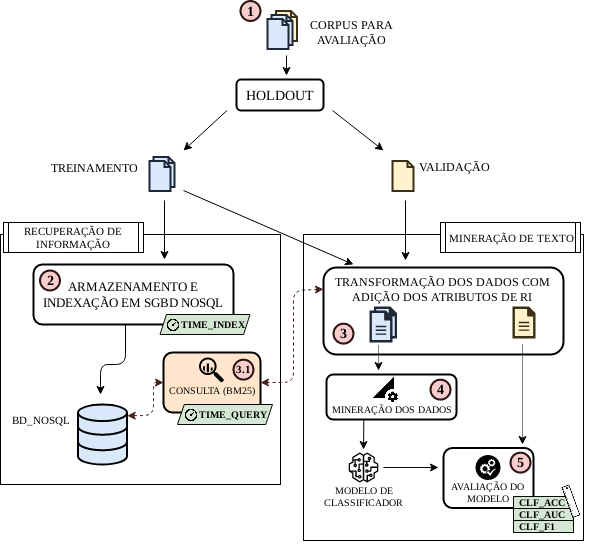
\includegraphics[width=0.8\textwidth]{img/diagrama-metodologia-v2-1.png}
    \end{center}
    \vspace{-0.5cm}
    \legend{\ABNTEXfontereduzida \textbf{Fonte:} O autor.}
    \label{fig:diagrama-cosulta-geração-atributos}
\end{figure}
    
    Cada exemplo do corpus a ser classificado é usado como consulta ao banco de dados NoSQL indexado, e cada uma destas consultas tem como resultado uma lista dos \textit{top-$k$} exemplos presentes no banco de dados, ordenada por pontuação de similaridade da função BM25, sendo esta pontuação calculada pela ferramenta de armazenamento indexação. 
    Esse procedimento está representado na Figura \ref{fig:diagrama-cosulta-geração-atributos}.
    
    O cálculo dos novos atributos é feito a partir da lista retornada dos \textit{top-$k$} exemplos, e são utilizadas as três funções de agregação sugeridas por \citeonline[p.~21--23]{WEREN_MESTRADO_2014}:
    \begin{enumerate*}[label=(\alph*)]
        \item média,
        \item soma, e
        \item contagem
    \end{enumerate*}, 
    levando em conta a classe binária da tarefa de classificação. 
    Assim, são gerados os atributos apresentados na Tabela \ref{tab:lista-atributos-sugeridos}.
    
    \begin{table}[H]
    \centering
    \begin{tabular}{|p{4.0cm}|l|l|}
        \hline
        \diagbox[width=4.4cm, height=2.0cm]{Agregação}{
            \raisebox{-1.3cm}{
                \rotatebox{90}{
                    \parbox{1.2cm}{\centering Exemplo}
                }
            }
        }  
        & \makecell[l]{Não faz parte da \\ classe da tarefa}
        & \makecell[l]{Faz parte da \\ classe da tarefa}
        \\ \hline
        \makecell[l]{Média aritmética \\ das pontuações}
        & \textbf{CLASS\_0\_BM25\_AVG} 
        & \textbf{CLASS\_1\_BM25\_AVG}  
        \\ \hline
        \makecell[l]{Contagem do número \\ de resultados}
        & \textbf{CLASS\_0\_BM25\_COUNT} 
        & \textbf{CLASS\_1\_BM25\_COUNT}  
        \\ \hline
        \makecell[l]{Soma das \\ pontuações}
        & \textbf{CLASS\_0\_BM25\_SUM} 
        & \textbf{CLASS\_1\_BM25\_SUM}  
        \\ 
        \hline
    \end{tabular}
    \caption{Atributos derivados de RI sugeridos.}
    \label{tab:lista-atributos-sugeridos}
\end{table}
    % Assim, serão geradas os seguintes atributos:
    % \begin{itemize}
    %     \item \textbf{CLASS\underscore{}0\underscore{}BM25\underscore{}AVG:} Média aritmética das pontuações dos resultados retornados pela consulta, que não fazem parte da classe da tarefa.
    %     \item \textbf{CLASS\underscore{}0\underscore{}BM25\underscore{}COUNT:} Contagem do número de resultados retornados pela consulta, que não fazem parte da classe da tarefa.
    %     \item \textbf{CLASS\underscore{}0\underscore{}BM25\underscore{}SUM:} Soma das pontuações dos resultados retornados pela consulta, que não fazem parte da classe da tarefa.        
    %     \item \textbf{CLASS\underscore{}1\underscore{}BM25\underscore{}AVG:} Média aritmética das pontuações dos resultados retornados pela consulta, que fazem parte da classe da tarefa.
    %     \item \textbf{CLASS\underscore{}1\underscore{}BM25\underscore{}COUNT:} Contagem do número de resultados retornados pela consulta, que fazem parte da classe da tarefa.
    %     \item \textbf{CLASS\underscore{}1\underscore{}BM25\underscore{}SUM:} Soma das pontuações dos resultados retornados pela consulta, que fazem parte da classe da tarefa.
    % \end{itemize}
    A definição do valor de \textit{top-$k$} altera diretamente os atributos gerados. 
    Contudo, a influência desta alteração não foi caso de estudo de Weren ao propor seus atributos de RI, e também nos seus estudos falta a informação de qual o valor de \textit{top-$k$} utilizado.
    A ferramenta de indexação utilizada nos estudos de Weren é o Zettair, e, quando não especificado explicitamente, o padrão de resposta a uma consulta é retornar 20 resultados.
    Então, utilizar \textit{top-$k = 20$} pode ser uma referência, no entanto o autor do presente estudo propõe-se a utilizar \textit{top-$k = 100$} para gerar os atributos de RI.
    
    
%  Por exemplo, para a classificação binária do PANCLEF 2019 Hyperpartisan podem ser criadas as variáveis a seguir:
% * avg_0 
% * count_0
% * sum_0
% * avg_1
% * count_1
% * sum_1

% baseadas no weren (2014)


\section{Medidas para avaliação de desempenho}  \label{sec:Medidas-para-avaliação-de-desempenho}
    São avaliados
    \begin{enumerate*}[label=(\alph*)]
        \item o desempenho das ferramentas utilizadas para indexação e consulta, por meio da avaliação temporal do desempenho computacional, e também
        \item o ganho de desempenho propiciado pelo uso dos atributos de RI em termos das medidas de classificadores de Mineração de Texto. % Essas medidas tem que ser citadas no referencial teórico.
    \end{enumerate*} 
    
    \subsection{Desempenho computacional das ferramentas}  \label{subsec:Desempenho-computacional}
        Para avaliar o desempenho das ferramentas de armazenamento e indexação são utilizadas duas medidas temporais:
        \begin{itemize}
            \item \textbf{TIME\underscore{}INDEX}: Tempo de execução para indexar o conjunto de treinamento de cada um dos corpus para avaliação elencados na Seção \ref{sec:Corpus-para-avaliação}. Dadas as 3 diferentes ferramentas de indexação e os 2 corpus selecionados, são computadas 6 TIME\underscore{}INDEX para comparação;
            
            \item \textbf{TIME\underscore{}QUERY}: Tempo para consulta de cada exemplo do conjunto de teste e geração dos atributos sugeridos na Seção \ref{sec:Atributos-de-RI-sugeridos} para o item específico. Dadas as 3 soluções para os dois corpus selecionados, e dadas as 3 ferramentas de indexação, 9 TIME\underscore{}QUERY são computadas.  
        \end{itemize}
        
        Essas variáveis serão computadas para cada uma das 3 ferramentas selecionadas sendo executadas no mesmo sistema computacional a fim de oferecer maior confiança aos números obtidos. 
        O sistema computacional utilizado para efetuar o experimento é especificado no capítulo de resultados.
    
% O teste de desempenho será feito comparando as ferramentas de indexação, tempo para indexar o treino de cada banco (TIME_TRN) em cada ferramenta.

% O tempo para consultar para cada linha do teste as variáveis a serem criadas (no caso de classificação binária iremos definir agregações do tipo count, sum e avg). Por exemplo, para a classificação binária do PANCLEF 2019 Hyperpartisan podem ser criadas as variáveis a seguir:
% * avg_0 
% * count_0
% * sum_0
% * avg_1
% * count_1
% * sum_1
    \subsection{Desempenho de classificador}  \label{subsec:Desempenho-de-classificador}
        O ganho de desempenho propiciado pelos atributos de RI criados é mensurado por medidas de desempenho de classificadores da literatura de mineração de dados, as mesmas também utilizadas na Mineração de Texto.
        Nesse estudo serão computadas as seguintes medidas:
        \begin{itemize}
            \item \textbf{CLF\underscore{}ACC}: Acurácia do classificador no conjunto de validação.
            \item \textbf{CLF\underscore{}F1}: $F_1$-score do classificador no conjunto de validação.
            
            % \item \textbf{CLF\underscore{}AUC}: Área sob a curva ROC.
    
            % Comentadas pois Rosalvo disse para ficar somente com acurácia (utilizada nas competições) e a área sob a curva ROC.
            % \item \textbf{CLF\underscore{}F1}: F1-Score
            % \item \textbf{CLF\underscore{}PRE}: Precisão do classificador.
            % \item \textbf{CLF\underscore{}REC}: Revocação do classificador.
        \end{itemize}
        A acurácia de um classificador, conforme apresentada na Subseção \ref{subsec:Medidas-de-avaliação-de-classificadores} definida pela Equação \ref{eq:medida-acurácia}, é a razão entre o número de exemplos classificados corretamente, e o número total de exemplos, no caso em questão, a variável \textbf{CLF\underscore{}ACC} a ser computada é referente ao conjunto de validação.
        O $F_1$-score é uma medida de classificador que engloba a precisão e revocação (ou sensitividade), e conforme apresentado na Subseção \ref{subsec:Medidas-de-avaliação-de-classificadores}, é uma boa medida da efetividade de classificadores em termos comparação pois engloba mais informação do que a acurácia. 
        É calculado conforme a definição dada pela Equação \ref{eq:medida-f-score} da Subseção \ref{subsec:Medidas-de-avaliação-de-classificadores}.
        
        
    
% Ao final será comparado o ganho de desempenho (acurácia, precisão, recall e F1-score) nas melhores soluções dos bancos definidos a partir da adição das variáveis criadas.
% Por exemplo para a PANCLEF 2019 Hyperpartisan será utilizada a solução que está disponível no github com melhor score e ela será executada novamente para conferir o resultado obtido de acurária que eles dizem e então será rodado novamente com a adição das variáveis de RI (BM25).

% \subsection{Subseção de exemplo 1 - Referenciando seções} \label{subsec:subsec1}






%--------------------------------------------------------------------------------------
% Insere a seção de cronograma
% Está comentada porque só é necessária no TCC I
%--------------------------------------------------------------------------------------
% %--------------------------------------------------------------------------------------
% Insere a seção de cronograma
%--------------------------------------------------------------------------------------

\section{Cronograma} \label{sec:Cronograma}

A Tabela \ref{tab:cronograma} mostra o cronograma de atividades a serem executadas para o Trabalho de Conclusão II (TCC II), com base no calendário do período 2019.2 da UNIVASF, definido pelo Calendário Acadêmico 2019 da instituição.

\begin{table}[!thb]
	%\huge
    \centering
    \caption{Cronograma das atividades previstas para o TCC II.}
    \begin{adjustbox}{max width=\textwidth}
    \begin{tabular}{p{6.5cm}|c|c|c|c|c|c}
        \toprule
        \textbf{Atividade}
        & Set & Out & Nov & Dez & Jan & Fev
        \\ \hline
        Definição e obtenção dos corpus para avaliação 
        & X   &     &     &     &     &          
        \\ \hline
        Inspeção e seleção das soluções com código fonte disponível
        & X   &     &     &     &     &          
        \\ \hline
        Instalação e familiarização com as ferramentas de arquivamento e indexação
        & X   & X   &     &     &     &          
        \\ \hline
        Indexação do conjunto de treinamento dos corpus
        &     & X   & X   &     &     &          
        \\ \hline
        Adição dos atributos de RI às soluções selecionadas
        &     & X   & X   &     &     &    
        \\ \hline
        Mineração dos dados por meio da reprodução das soluções selecionadas com/sem adição dos atributos de RI
        &     &     & X   & X   & X   &  
        \\ \hline
        Escrita do TCC II                       
        & X   & X   & X   & X   & X   &         
        \\ \hline
        Defesa do TCC II                        
        &     &     &     &     & X   &        
        \\
        \bottomrule
    \end{tabular}
    \end{adjustbox}
    
    \label{tab:cronograma} 
    % \legend{\textbf{Fonte:} O autor.}
\end{table}
